% Source material: docs/seminar/reproducibility-evidence-v1.md
% See also: docs/seminar/audit.md — validation sections
% Figures: copy scripts/figures/*.png → thesis/figs/results/ before compiling

\chapter{Results}
\label{ch:results}

% ============================================================
\section{TractoInferno Validation}
\label{sec:results-tractoinferno}
% ============================================================

\subsection{Dataset and Setup}
\label{subsec:tractoinferno-setup}

% TODO: Describe the TractoInferno dataset: 167 subjects from OpenNeuro ds003900 (trainset),
%       csttool v0.4.1 (git commit 1433ac4), 334 hemisphere comparisons total,
%       330 valid (98.8% success rate), 4 excluded (reasons: INVALID_SPACE / E_CAND_MISSING).
%       State that each subject was processed using a single csttool run command with
%       fixed parameters (fa-thr 0.2, seed-density 2, seed 42).

\subsection{Spatial Overlap}
\label{subsec:tractoinferno-dice}

% TODO: Report Dice mean ± SD (0.283 ± 0.065), median 0.285, range [0.053, 0.471].
%       Left hemisphere: 0.268 ± 0.066. Right hemisphere: 0.299 ± 0.060.
%       Mention the two figures below.

\begin{figure}[ht]
    \centering
    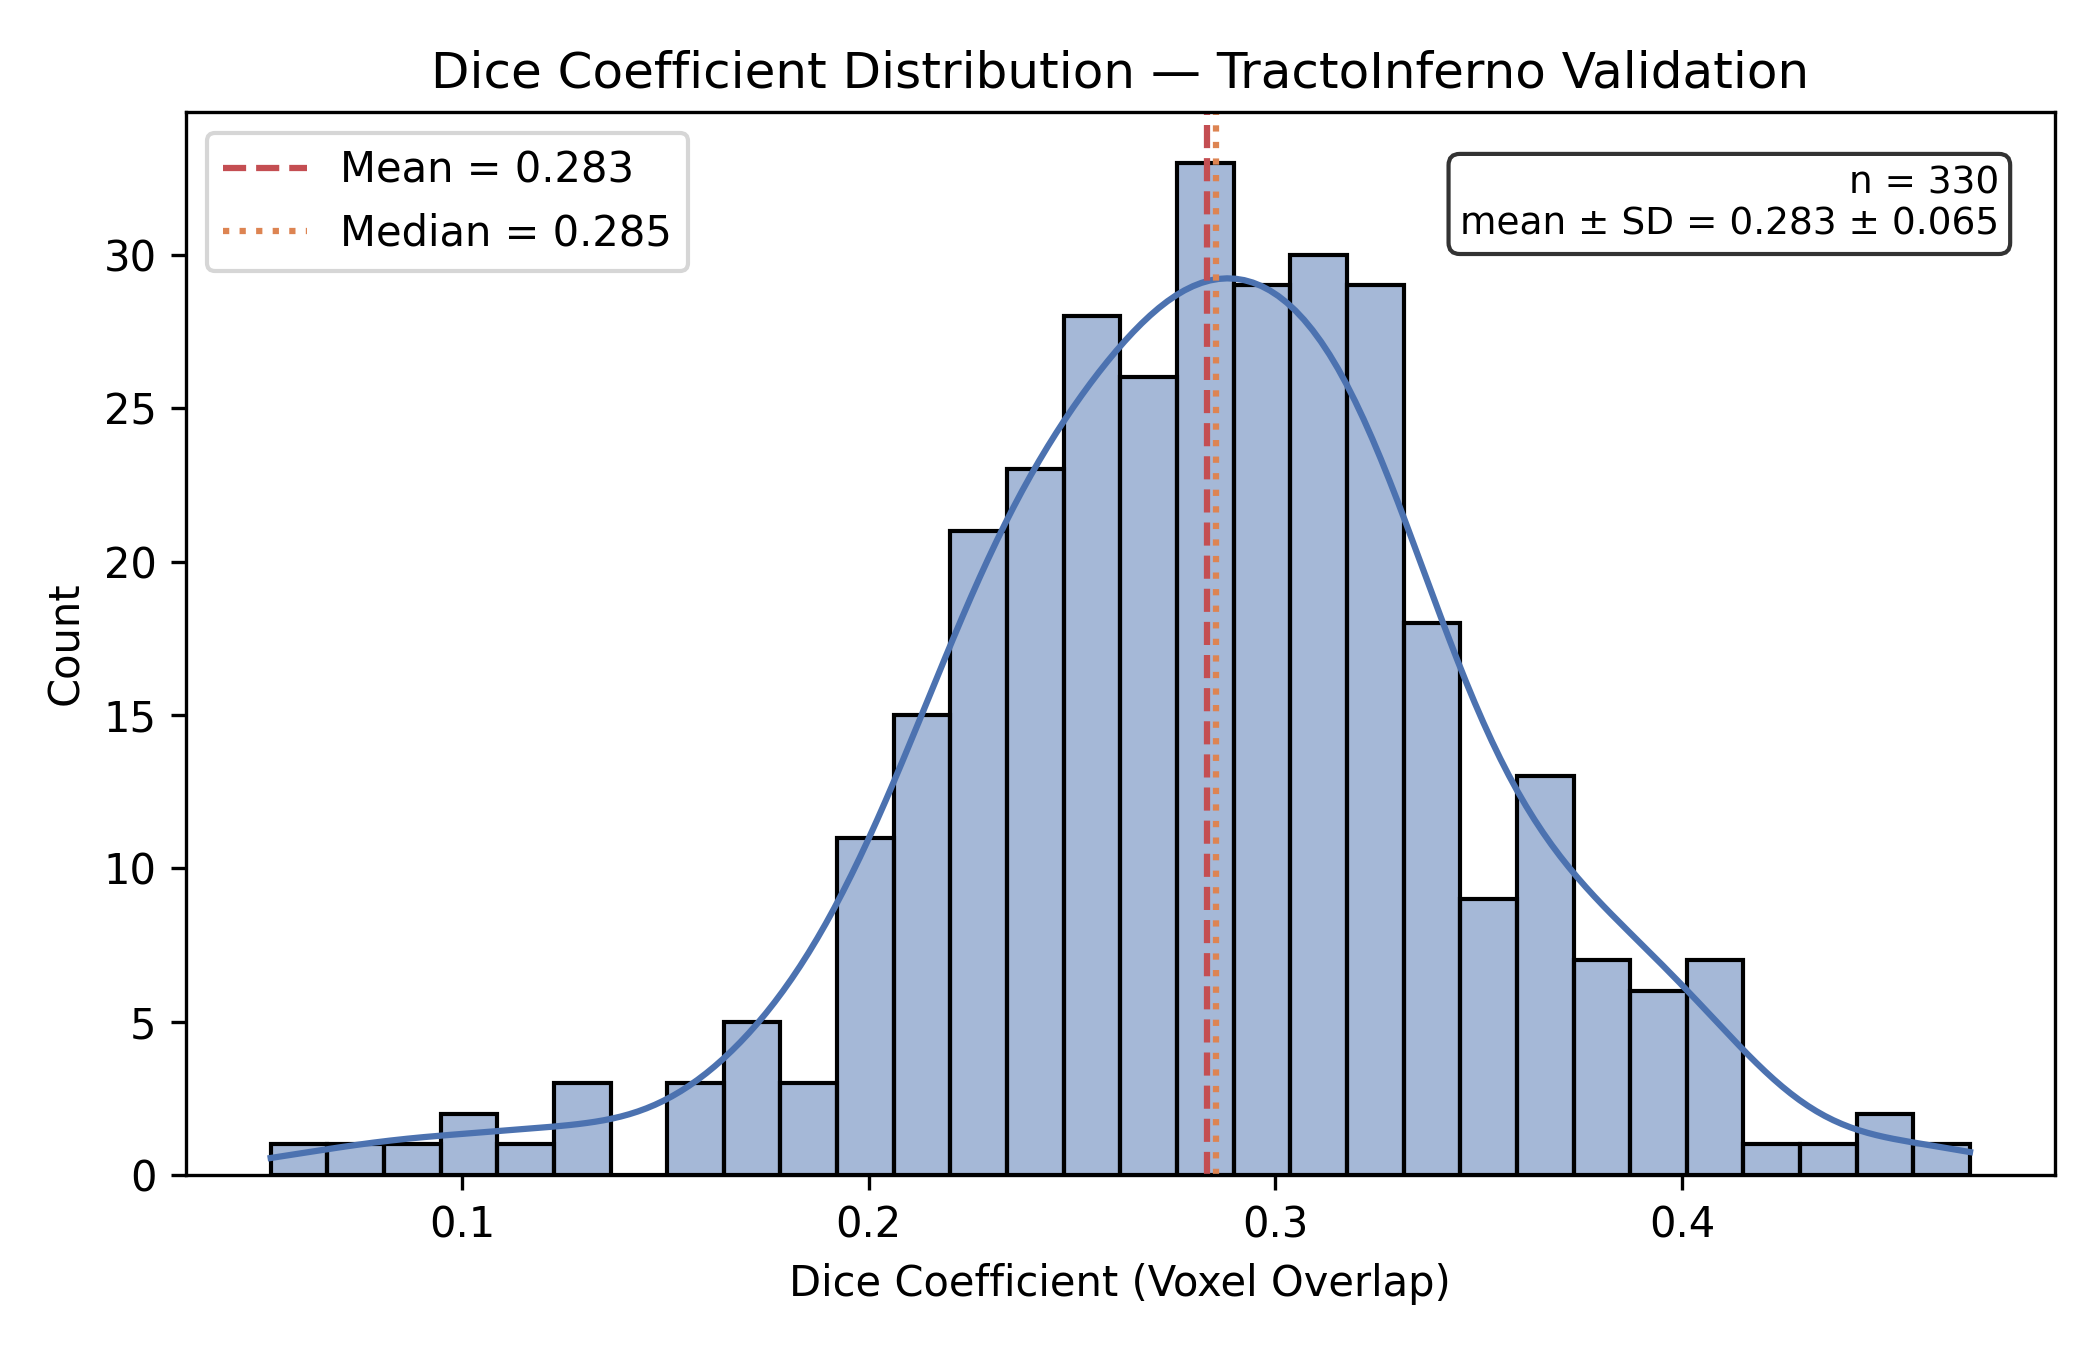
\includegraphics[width=0.9\linewidth]{figs/results/dice_distribution.png}
    \caption{Distribution of Dice similarity coefficients across 330 valid hemisphere
             comparisons (TractoInferno trainset, $n = 167$ subjects).}
    \label{fig:dice-distribution}
\end{figure}

\begin{figure}[ht]
    \centering
    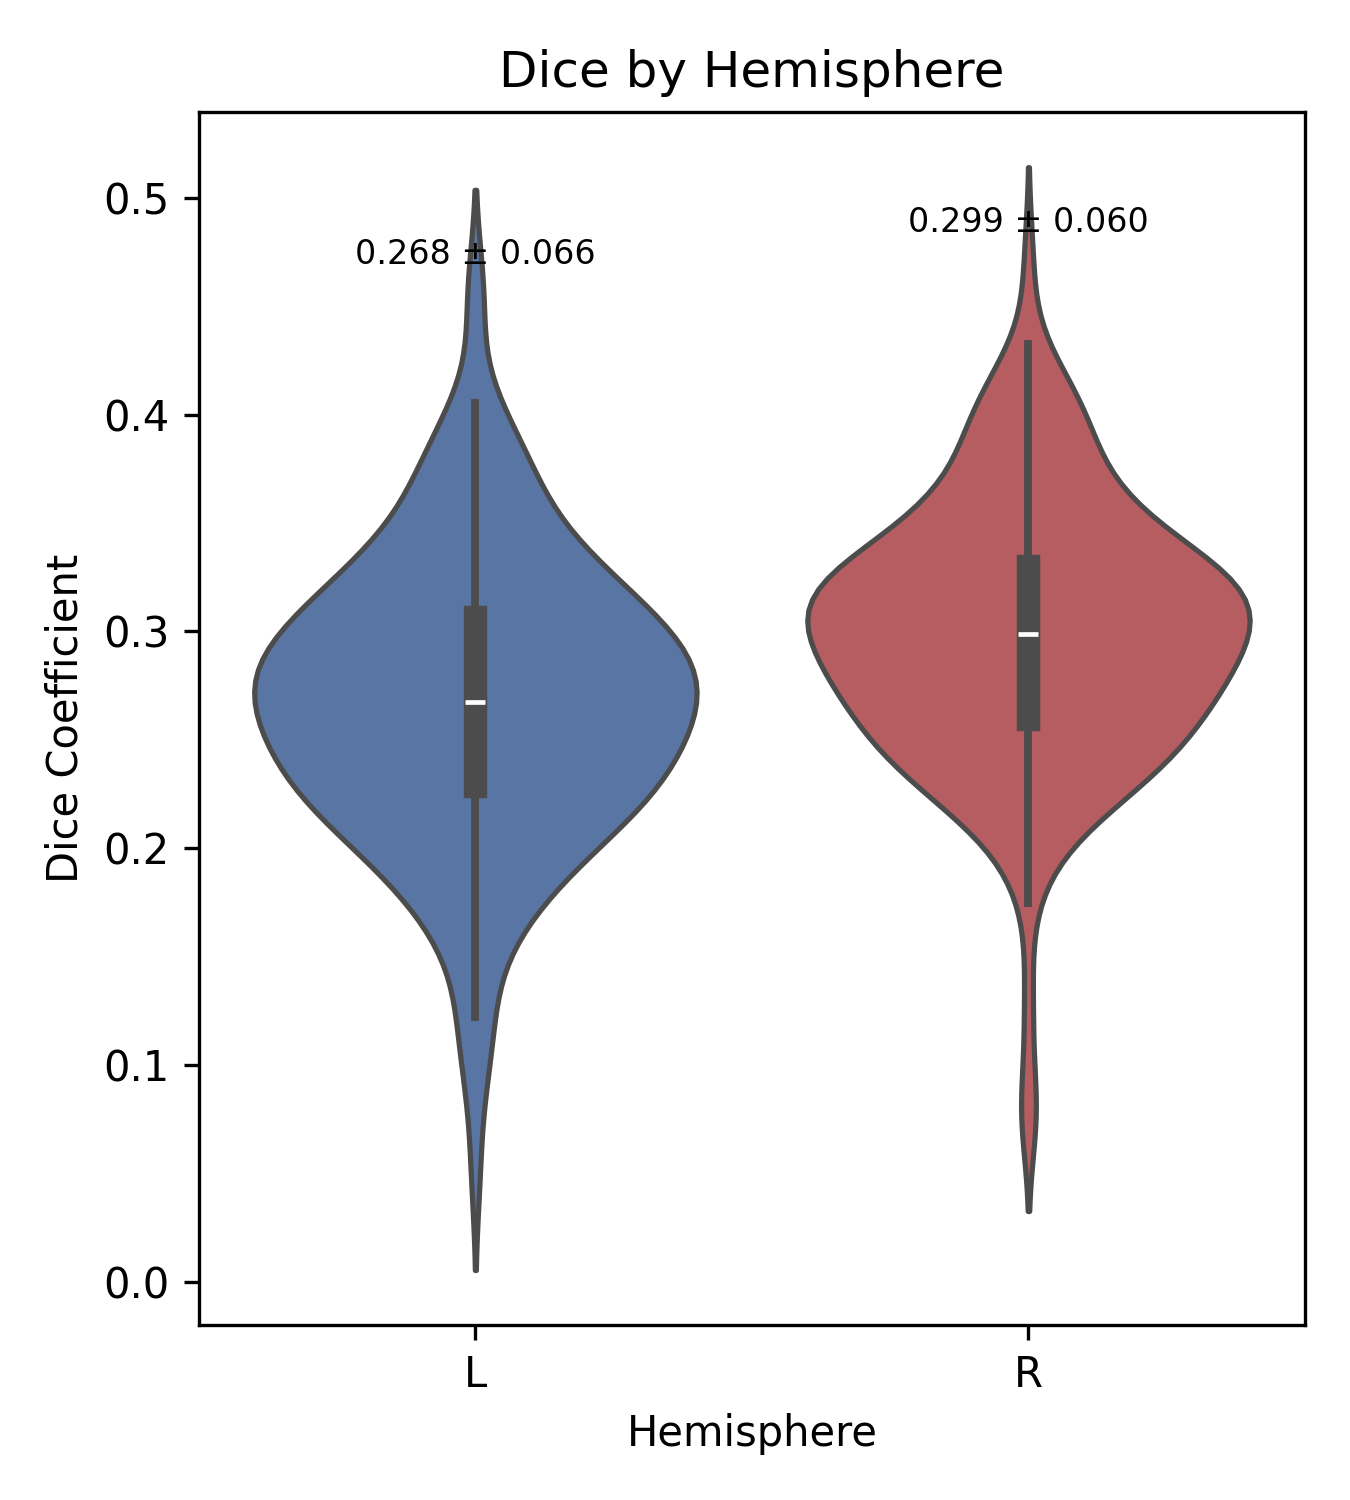
\includegraphics[width=0.9\linewidth]{figs/results/dice_by_hemisphere.png}
    \caption{Dice coefficients split by hemisphere. Right CST (mean 0.299) consistently
             yielded higher overlap than left CST (mean 0.268).}
    \label{fig:dice-by-hemisphere}
\end{figure}

\subsection{Precision and Recall}
\label{subsec:tractoinferno-precision-recall}

% TODO: Precision mean ± SD: 0.854 ± 0.066. Recall mean ± SD: 0.172 ± 0.047.
%       Note that the asymmetry (high precision, low recall) is expected given the
%       streamline count difference (see below and Discussion). Do not interpret here
%       beyond a brief quantitative note — leave interpretation for Discussion.

\begin{figure}[ht]
    \centering
    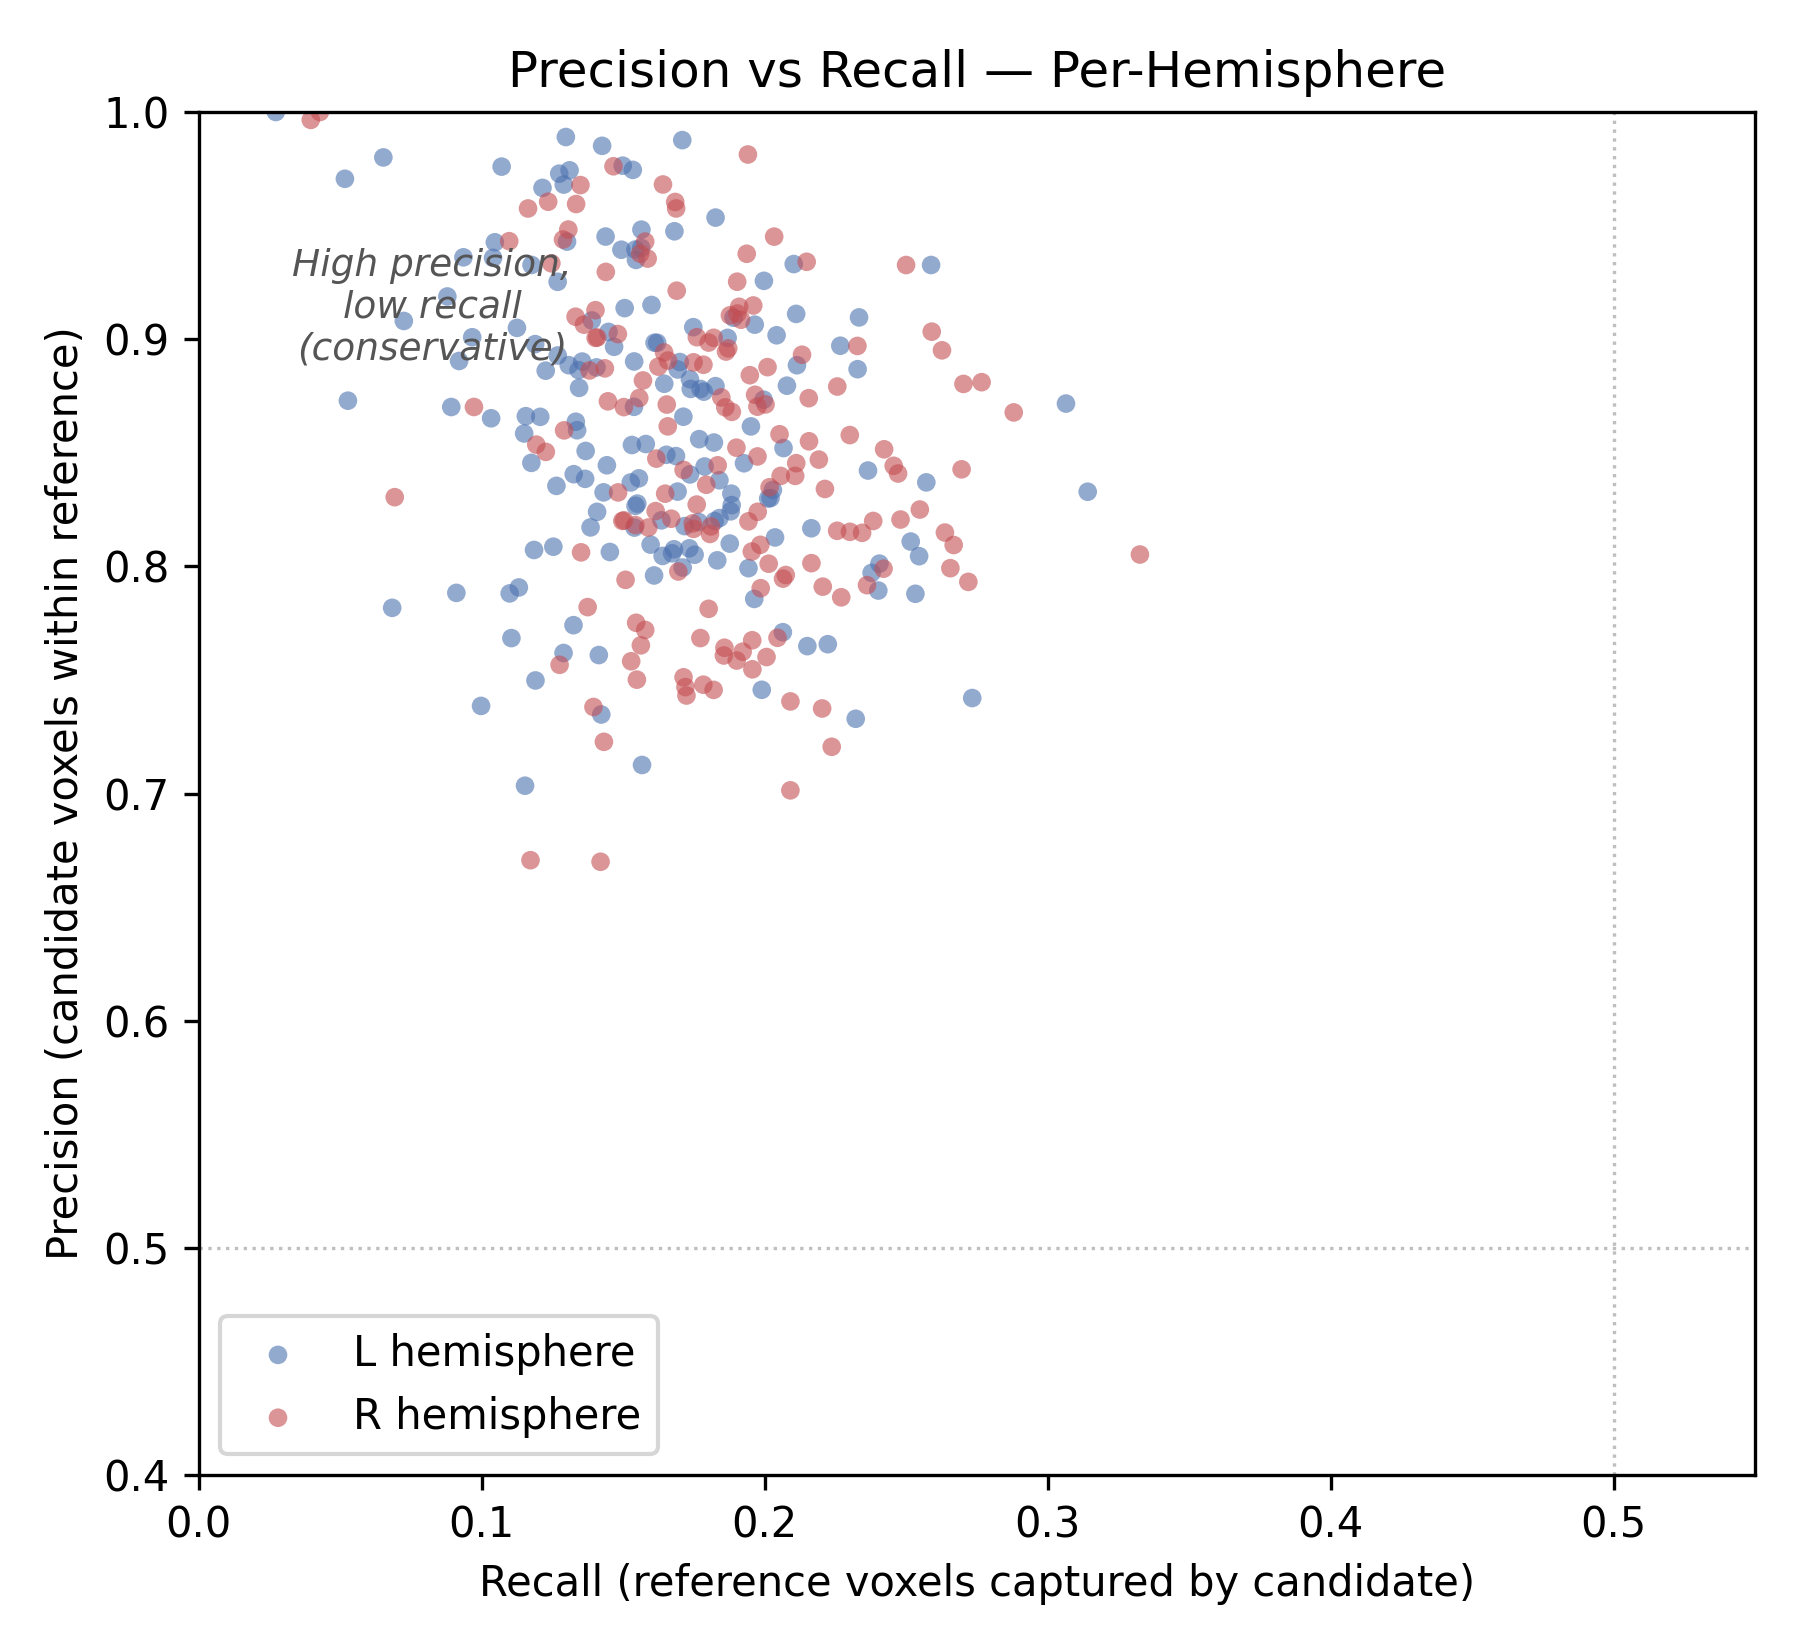
\includegraphics[width=0.9\linewidth]{figs/results/precision_recall.png}
    \caption{Precision and recall per subject for left and right CST across all
             330 valid comparisons.}
    \label{fig:precision-recall}
\end{figure}

\subsection{Streamline Counts}
\label{subsec:tractoinferno-streamlines}

% TODO: Candidate (csttool) mean 4,093 streamlines per bundle (range 358–9,676).
%       Reference (TractoInferno) mean 61,188 (range 19,244–169,699).
%       Approximately 15× fewer streamlines than the probabilistic reference.
%       This is a direct consequence of deterministic single-peak tracking and is
%       discussed in Section~\ref{sec:discussion-dice}.

\begin{figure}[ht]
    \centering
    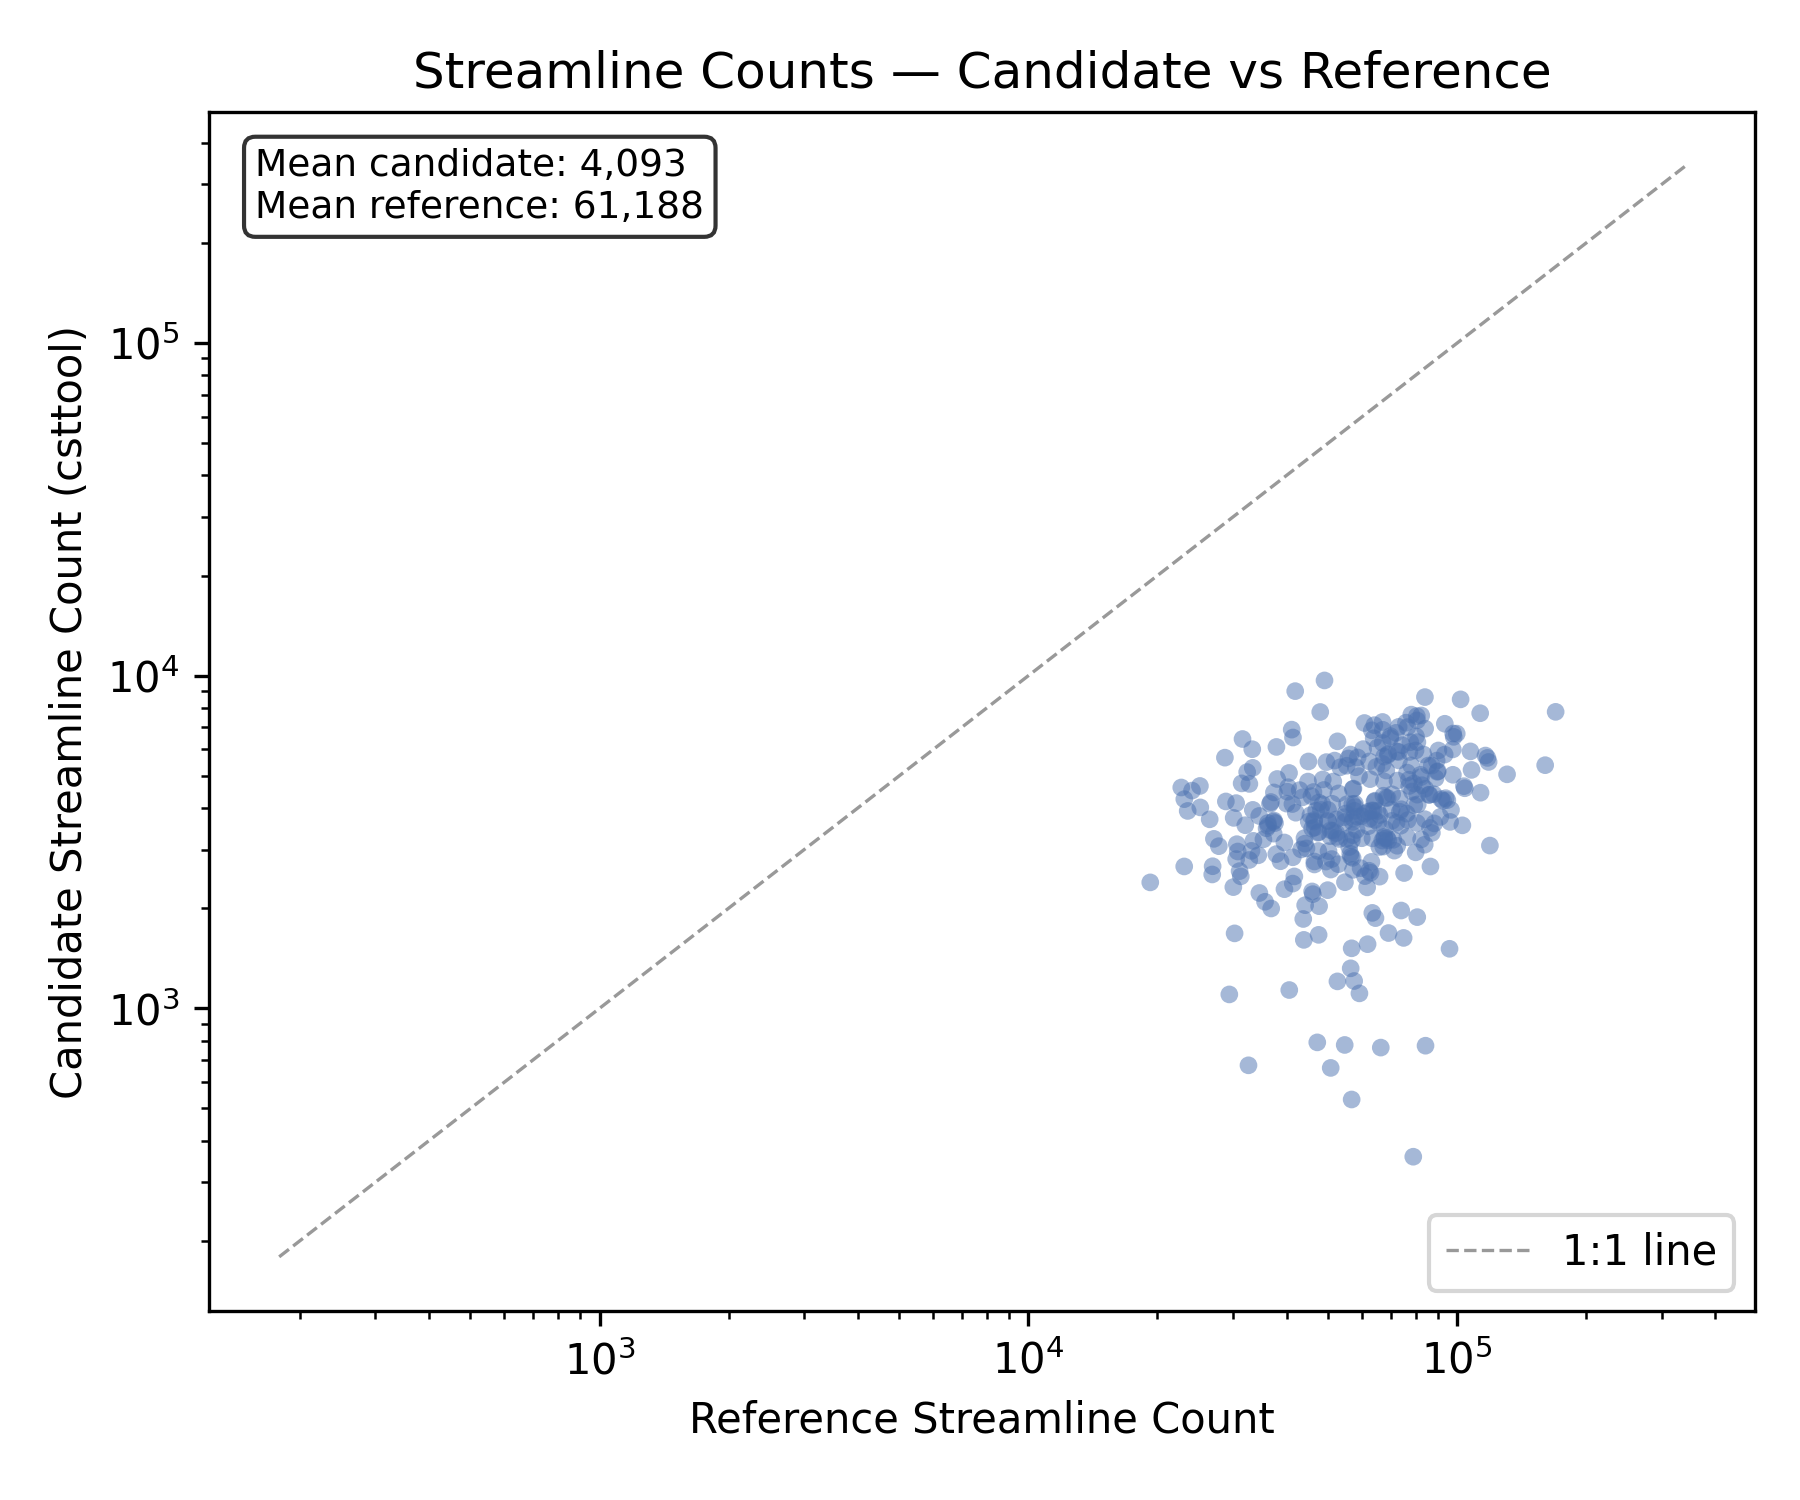
\includegraphics[width=0.9\linewidth]{figs/results/streamline_counts.png}
    \caption{Per-subject streamline counts for csttool candidates vs.\ TractoInferno
             reference bundles (log scale). The \(\approx\)15$\times$ difference is inherent
             to deterministic vs.\ probabilistic tracking methodology.}
    \label{fig:streamline-counts}
\end{figure}

\begin{figure}[ht]
    \centering
    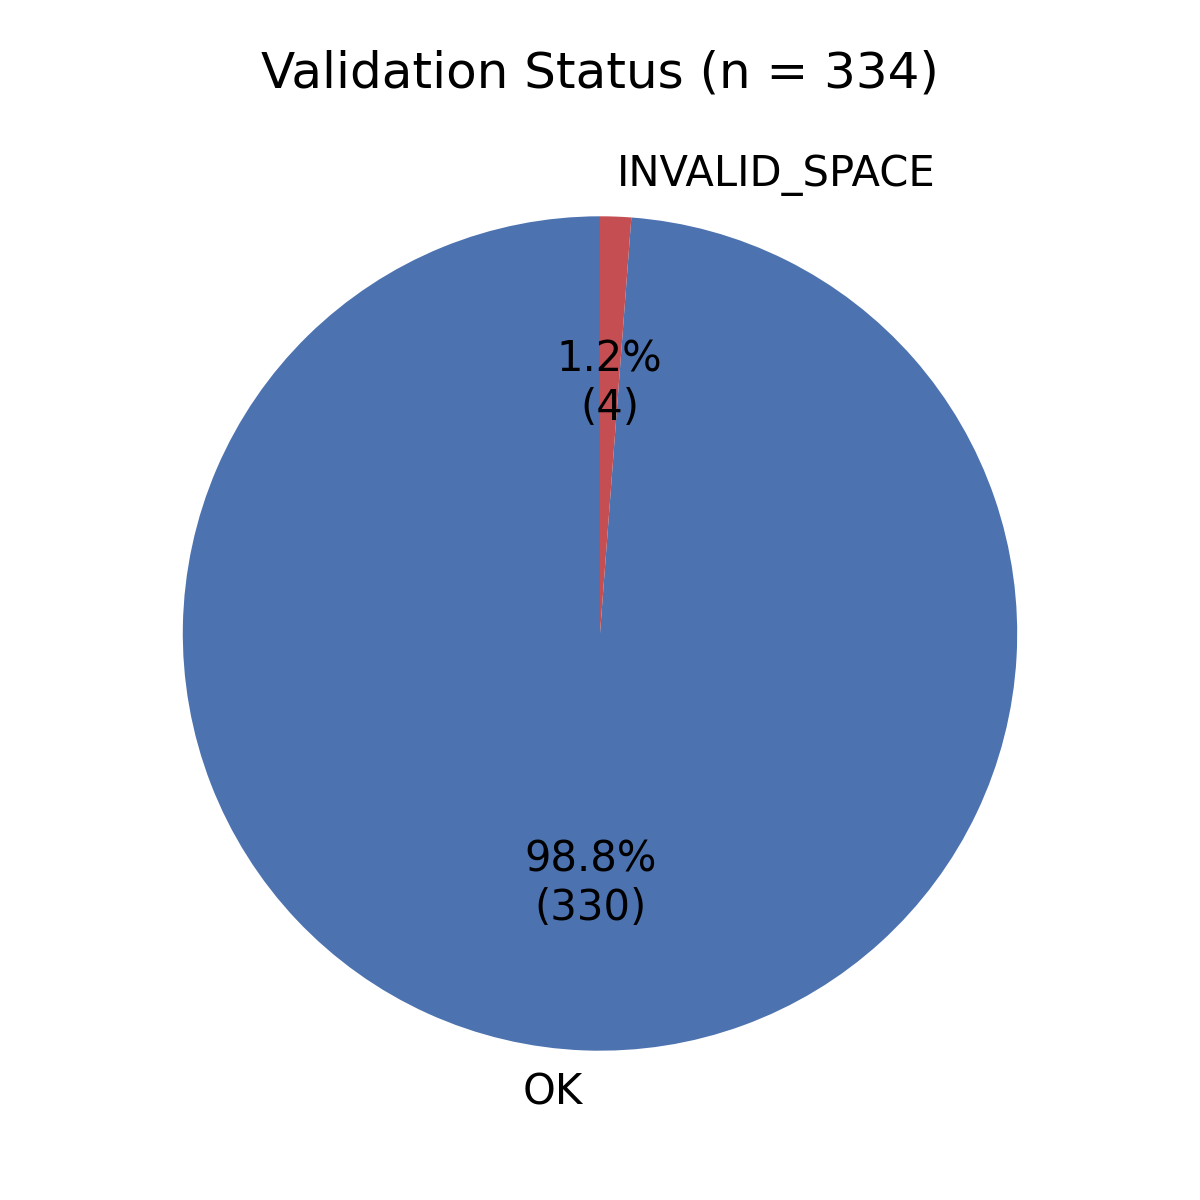
\includegraphics[width=0.9\linewidth]{figs/results/success_rate.png}
    \caption{Processing success rate across the TractoInferno trainset. 330 of 334
             hemisphere comparisons (98.8\%) completed successfully.}
    \label{fig:success-rate}
\end{figure}

% ============================================================
\section{Determinism Validation}
\label{sec:results-determinism}
% ============================================================

\subsection{Setup}
\label{subsec:determinism-setup}

% TODO: Three repeated runs per subject with identical parameters: seed=42, threading
%       pinned to 1 CPU (OMP_NUM_THREADS=1), csttool v0.4.1. Preprocessing was performed
%       once; all three runs consumed the same fixed preprocessed NIfTI as input.
%       Outputs compared bitwise (SHA-256 of tractograms, scalar maps, metrics CSVs, reports).

\subsection{Single-Subject Test}
\label{subsec:determinism-single}

% TODO: Subject sub-1204 (3T scanner, 32 gradient directions, 1 mm isotropic voxels).
%       Whole-brain: 575,111 streamlines. CST-L: 3,243 streamlines. CST-R: 4,038 streamlines.
%       Scalar map dimensions: 134×178×136 voxels (FA, MD, RD, AD).
%       Result: all outputs bitwise identical across all 3 runs — tractograms, scalar maps,
%       per-tract metrics, and PDF reports.

\begin{figure}[ht]
    \centering
    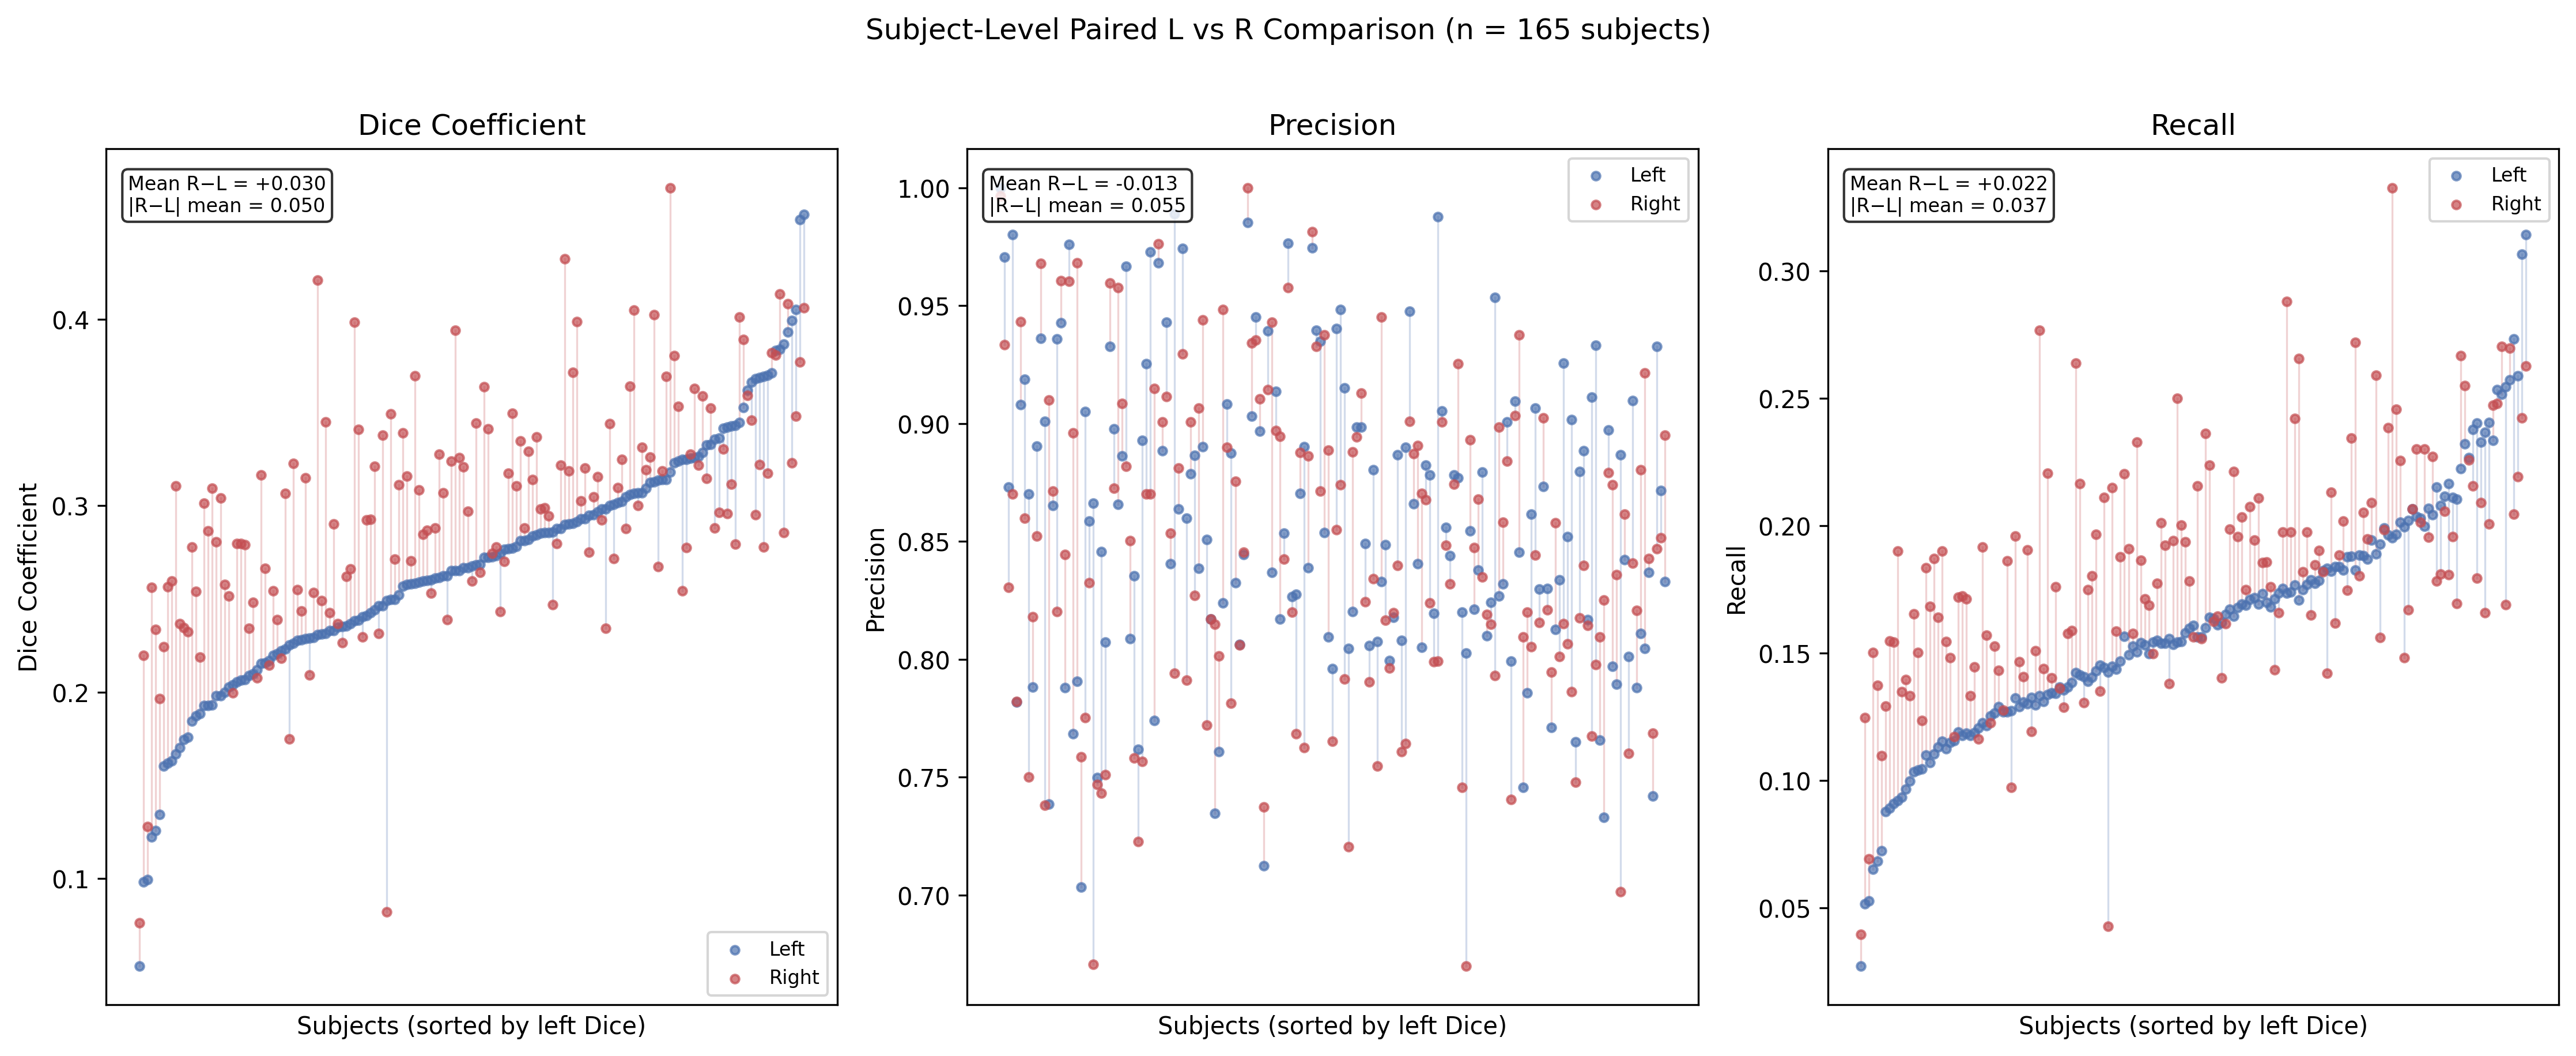
\includegraphics[width=0.9\linewidth]{figs/results/subject_paired.png}
    \caption{Paired CST metrics (FA mean, streamline count) across three repeated runs
             for sub-1204. Overlapping points confirm bitwise identical outputs.}
    \label{fig:subject-paired}
\end{figure}

\subsection{Multi-Subject Test}
\label{subsec:determinism-multi}

% TODO: Five subjects: sub-1007, sub-1030, sub-1165, sub-1204, sub-1276. Three runs each
%       (15 total pipeline executions). Overall verdict: BITWISE_IDENTICAL for every subject.
%       Report the subject-level breakdown if available from the determinism summary CSV.
%       This demonstrates that determinism is a general property of the pipeline, not a
%       single-case artifact.
